\subsection{LHCb at the LHC}
LHCb is one of the four large experiments at the LHC.
The LHC is a $pp$ collider with a much higher center of mass energy compared to
any $e^-e^+$ collider.

% Talk about subdetectors
LHCb is a single-arm spectrometer.
Its constituent subdetectors, from closest to farthest from the collision point,
are shown in \autoref{fig:lhcb_detector_view}:
The Vertex Locator (VELO) provides precise measurements of track coordinates
close to the collision point.
Two Ring Imaging Cherencov counters (RICH1, RICH2) provide particle
identification for charged particles over a wide range of momentum.
Tracker Turicensis (TT) and Inner Tracker (IT) provide additional tracking for
charged particles.
The Outer Tracker (OT) is used for tracking, as well as measures the momentum
of charged particles.
The calorimeters (ECAL and HCAL) have a first-level (L0) trigger to select
hadron, electron, and photon candidates based on their transverse momentum
$p_T$;
they also provide identification for the particles listed above;
finally, they provide energy and position measurements for these particles.
The farthest subdetector is Muon system (M1-5);
it provides L0 high $p_T$ muon trigger, and a high-level trigger (HLT) for muon
identification \cite{LHCb:2008}.

\begin{figure}[ht]
    \centering
    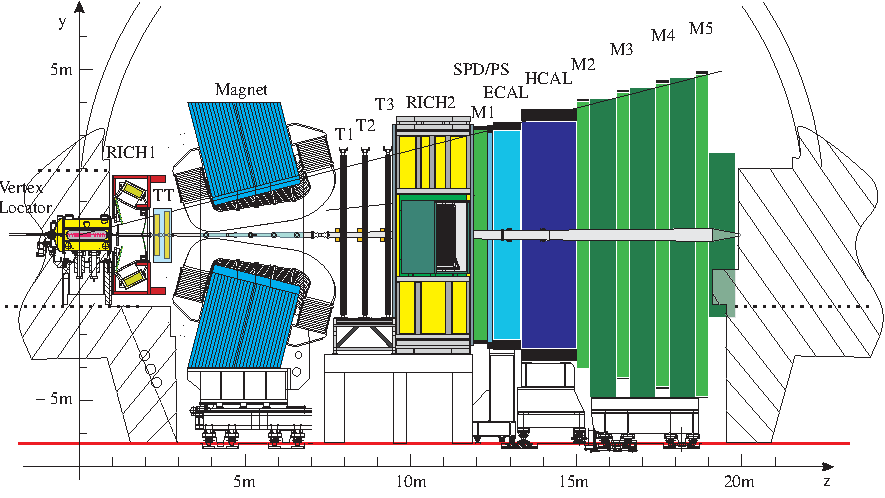
\includegraphics[width=0.7\textwidth]{figs/lhcb_detector_view.pdf}
    \caption{
        View of the LHCb detector.
        Vertex Locator (VELO) is closest to collision point.
    }
    \label{fig:lhcb_detector_view}
\end{figure}

% Talk about the LHC being a hadron collider and the difficulties associated
% with it
Unlike electron, proton is a composite particle, made of $u, u, d$ quarks.
At the energy scale of the LHC, it is easy to see from the parton distribution
functions\footnote{
    Number density to find fraction of the momentum (denoted as $x$) at certain
    squared energy scale $Q^2$.
} that there are plenty of other elementary particles, such as gluons, that can
participate in the collision.
These particles may carry varying portion of the total
momentum \cite{Ball:2014uwa}.

Effectively, partons are being collided.
This results in a very frequent and noisy background---Comparing to \BaBar/, one
notable addition of the LHCb is the triggering system, which is used to reduce
the readout rate \cite{LHCb:2008}.
In other words, we cannot afford to store all uninteresting events
(backgrounds).
Also, since we do not know the precise fraction of momentum carried by
interactive partons\footnote{
Again, these are characterized by parton distribution functions}, no kinematic
restriction can be applied directly.

It is obvious that $e^- e^+$ colliders provide a \emph{much} cleaner background.
However, the LHC generates much more $b\bar{b}$\footnote{
    Note that this is \emph{not} necessarily \Y4S/.
} events compared to \BaBar/, due to a much larger cross section.
At \SI{13}{TeV}, the measured cross section at LHCb\footnote{
    For $2 < \eta < 5$ only, since this is the LHCb acceptance range.
} is $144 \pm 1 \pm 21$~\si{\mu b} \cite{Aaij:2016avz}.
% FIXME: Is the calculation for BaBar cross section legal?
Use the integrated luminosity and total number of $B\overline{B}$ events
contained in the on-resonance \Y4S/ sample, we compute the $b\bar{b}$ cross
section of \BaBar/ to be $\approx 1.09$~\si{nb}, which is much smaller than that
of the LHCb.

% Talk about LHCb being forward-only
Another interesting design choice is the geometry of the LHCb detector:
Instead of a barrel $4\pi$ detector, it is a forward-only spectrometer.
At high energy, $b\bar{b}$ production is mostly produced
in the forward and backward direction.
The LHCb design is a very cost-effective way to construct a detector at the LHC
dedicated for $B$ physics \cite{LHCb:2008}.

% Talk about tracking
LHCb has a spectacular tracking and vertexing system---In some cases, it is even
better than that of \BaBar/.
The spatial resolution of VELO is about \SI{6}{\mu m};
For TT and IT, about \SI{50}{\mu m} \cite{LHCb:2008}.

% Talk about ECAL, which is not the best in the world
On the other hand, the calorimeters are mediocre.
The energy resolution of the ECAL and HCAL are:
\begin{align*}
    \frac{\sigma_E}{E}_{ECAL} &= \frac{(8.5-9.5)\%}{\sqrt{E}}
        \oplus (9 \pm 2)\% \\
    \frac{\sigma_E}{E}_{HCAL} &= \frac{(69 \pm 5)\%}{\sqrt{E}}
        \oplus (9 \pm 2)\% \\
\end{align*}
with $E$ in \si{GeV} \cite{Guz:2017}.

% Talk about run 1 and run 2 luminosity
LHCb collected data from 2010 to 2012 (Run 1), and 2015 to 2018 (Run 2).
An incomplete integrated luminosity (summing from 2010 to 2017) is
\SI{6.829}{fb^{-1}} \cite{LHCb-Facts:2019}.

% Talk about LS2 upgrade and LHCb's future
Currently, LHCb is shut down for an upgrade.
We, the University of Maryland group, are actively participating in the upgrade.
Specifically, we are designing data transmission system as well as power
delivery system for the Upstream Tracker (UT) upgrade, which will replace the TT
in Run 3.

The current TT system limits the readout rate to \SI{1}{MHz}, due to the L0
hardware trigger.
The updated UT will have a \SI{40}{MHz} rate, which will make a fully
software-based trigger possible \cite{LHCbCollaboration:2014tuj}.
Another benefit is to reduce ghost tracks\footnote{
    Ghost tracks are formed by linking VELO tracks with the wrong downstream
    tracks.
} by providing additional measurements between VELO and downstream trackers
(currently IT, will be replaced by SciFi tracker) \cite{Parker:2017}.
